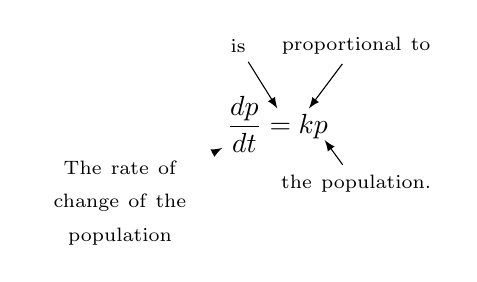
\begin{tikzpicture}[>=latex]
%\draw [thin,step=1cm] (0,0) grid  (3,3);
\draw  (1,1) node {$\displaystyle \frac{dp}{dt} = kp$};

\draw [{\colorone}] (-1,0) node [text width=60pt,align=center](a) {\scriptsize \centering The rate of change of the population};
\draw [{\colorone},->] (a) -- (.3,.7);

\draw [{\colorone}] (2,.25) node [text width=60pt,align=center] (b) {\scriptsize \centering the population.};
\draw [{\colorone},->] (b) -- (1.6,.8);

\draw [{\colorone}] (.5,2) node [text width=32pt,align=center] (c) {\scriptsize \centering is};
\draw [{\colorone},->] (c) -- (1,1.2);

\draw [{\colorone}] (2,2) node [text width=60pt,align=center] (d) {\scriptsize \centering proportional to};
\draw [{\colorone},->] (d) -- (1.4,1.2);

\end{tikzpicture}
